\documentclass[11pt]{report}

\usepackage[frenchb]{babel}
\usepackage[utf8]{inputenc}
\usepackage[T1]{fontenc}
\usepackage{charter}
\usepackage{graphicx}
\usepackage{amsmath}
\usepackage{amsfonts}
\usepackage{stmaryrd}
\usepackage{diagbox}
\usepackage{amsthm}
\usepackage{textcomp}
\usepackage[a4paper,margin=1in]{geometry}
\setcounter{MaxMatrixCols}{20}

\usepackage{float}
\usepackage{empheq}
\usepackage{siunitx}

\usepackage{url}

% \setlength{\voffset}{-0.75in}
% \setlength{\headsep}{5pt}
\usepackage{mathtools}

\setcounter{tocdepth}{1}

\setlength{\parindent}{0em}
\setlength{\parskip}{0.5em}

\DeclarePairedDelimiter\abs{\lvert}{\rvert}%
\DeclarePairedDelimiter\norm{\lVert}{\rVert}%
\newcommand{\boxedeq}[2]{\begin{empheq}[box={\fboxsep=6pt\fbox}]{align}\label{#1}#2\end{empheq}}

\makeatletter
\let\oldabs\abs
\def\abs{\@ifstar{\oldabs}{\oldabs*}}
%
\let\oldnorm\norm
\def\norm{\@ifstar{\oldnorm}{\oldnorm*}}
\makeatother

\newtheorem*{remark}{Remarque}
\newtheorem*{lemma}{Lemme}

\begin{document}
\begin{titlepage}
	\centering
	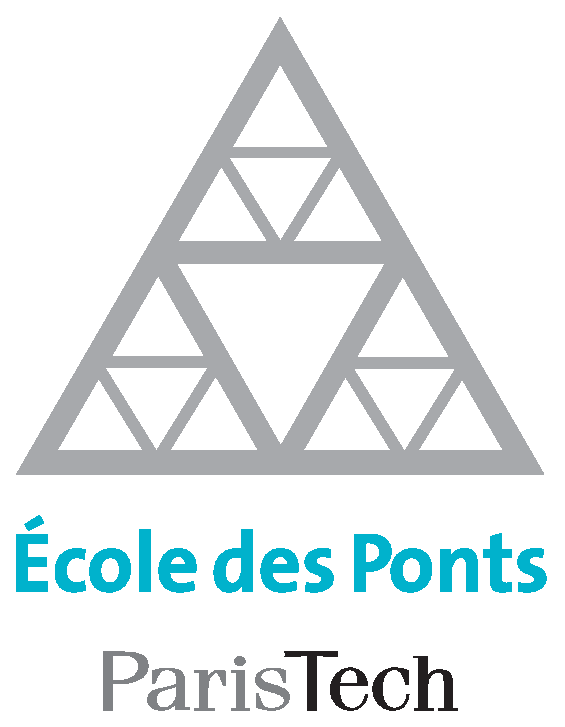
\includegraphics[width=0.15\textwidth]{logo-enpc.eps}\par\vspace{1cm}
	{\scshape\LARGE École des Ponts ParisTech \par}
	\vspace{1cm}
	{\scshape\Large Projet d'initiation à la recherche 2016 \par}
	\vspace{1cm}
	{\Large {\scshape Cours d'ouverture 1A : } \\ Imagerie numérique -- Application en mécanique des matériaux \par}
	\medskip
	{\Large\itshape Mathieu Aubry (LIGM-Imagine) -- Michel Bornert (Navier) \\ Patrick Aimedieu (Navier) -- Marie Bonnet (Navier) \par}
	\vspace{1.5cm}
	{\huge\bfseries Mesure de forme et de déformation par imagerie numérique \par}
	{\Large Reconstruction d’un objet centimétrique par acquisition et corrélation d’images \par}
	\medskip
	{\Large\itshape Joar Chouaki -- Mathieu Lerouge -- Aurélie Shi -- Louis Trezzini\par}
	\medskip
	{\large 26 mai 2016 \par}

	\vfill
	\begin{minipage}{16cm}
    {\normalsize
     \parindent=0pt
     {\scshape Résumé :} L’objectif de notre projet est de développer un procédé permettant de déterminer la géométrie tridimensionnelle d’un objet centimétrique à partir d'une séquence de photos obtenue à l'aide d'une unique caméra. Un tel procédé se compose de trois étapes principales : l'acquisition de photos de l’objet dans différentes configurations, la mise en correspondance des points entre les différentes captures et la reconstruction tridimensionnelle de l’objet - celle-ci dépendant du modèle de caméra choisi ainsi que de la qualité de la calibration. Aussi, une fine précision de la reconstruction étant attendue, il est essentiel d'évaluer de façon quantitative le bruit et la propagation d'erreurs à chaque étape du procédé.
     \par
    }
    \end{minipage}

    \medskip

    \begin{minipage}{16cm}
    {\normalsize
    \parindent=0pt
        {\scshape Mots-clés :} Imagerie, \emph{structure from motion}, corrélation, triangulation, calibration de caméra
    \par}
    \end{minipage}
\end{titlepage}

\tableofcontents

\chapter*{Introduction}
\addcontentsline{toc}{chapter}{Introduction}

La tomographie à rayons X est une technique d'imagerie qui permet d'observer des échantillons en trois dimensions, avec une très haute résolution, de manière non destructive. Elle repose sur l'analyse de l'interaction entre un faisceau de rayons X et l'échantillon étudié. Le tomographe se compose essentiellement:
\begin{itemize}
    \item d'une source de rayons X,
    \item d'une platine de rotation très précise sur laquelle est placé l'échantillon étudié,
    \item d'un détecteur de rayons X plan.
\end{itemize}

L'échantillon est soumis au faisceau de rayons X suivant différentes positions angulaires. Pour chacune d'entre elles, le détecteur enregistre le rayonnement transmis. Puis, à partir de ces enregistrements successifs, un algorithme de reconstruction fournit l'image tridimensionnelle de l'échantillon sous forme de coupes successives.

Le microtomographe dont dispose le laboratoire Navier possède de nombreuses applications. Par exemple, il permet, par reconstructions successives, de suivre l'évolution d'un échantillon soumis à des sollicitations. Néanmoins, le temps nécessaire à ces reconstructions est important (de l'ordre de plusieurs heures) et il peut parfois être nécessaire d'observer des phénomènes en surface (tels que les glissements dans le cas de matériaux composites), ce que le tomographe ne permet pas. C'est ce besoin qui a motivé la naissance de notre projet.

L'objectif de ce projet ambitieux est donc d'élaborer un montage, un protocole et des programmes permettant d'obtenir une reconstruction tridimensionnelle de la surface de l'échantillon. Il s'agit également de réaliser une analyse précise des erreurs propres aux différentes étapes du projet afin de pouvoir évaluer les incertitudes sur les mesures.

\chapter{Modèles de caméra}

Afin de résoudre le problème de triangulation et de reconstruction 3D de l'objet, nous devons adopter un modèle géométrique pour décrire la scène et les caméras.

\section{Le modèle de caméra orthographique avec échelle, plus adapté aux grandes focales}

Nous choisissons aussi d'étudier le modèle de caméra orthographique avec échelle, qui est une approximation de la caméra perspective. Elle consiste à d'abord projeter orthogonalement les points sur un plan choisi (on décide de prendre le plan $Z$ moyen), puis d'effectuer une projection perspective du premier projeté. Cette approximation permet de s'abstraire de toutes les non-linéarités, mais nécessite, pour être précise, que le relief soit petit devant la distance lentille-objet. \cite{poelman1993paraperspective}

On considère les notations suivantes :

On peut alors écrire la projection du point $P^i$ sur la caméra $c$ :

$$ p_c^i = \frac{f_c}{t_c^z} \big[ \begin{pmatrix} i_c^T \\ j_c^T \end{pmatrix} P^i + \begin{pmatrix} t_c^x \\ t_c^y \end{pmatrix} \big] = \big[ \begin{pmatrix} m_c^T \\ n_c^T \end{pmatrix} P^i + \begin{pmatrix} {t'}_c^x \\ {t'}_c^y \end{pmatrix} \big]  $$

Pour $N$ points et $C$ caméras :

$$
W =
\begin{pmatrix}
p_1^1 & \dots & p_1^N \\ \vdots & & \vdots \\ p_C^1 & \dots & p_C^N
\end{pmatrix}
=
\begin{pmatrix}
m_1^T \\ n_1^T \\ \vdots \\ m_C^T \\ n_C^T
\end{pmatrix}
\begin{pmatrix}
P^1 & \dots & P^N
\end{pmatrix}
+
\begin{pmatrix}
{t'}_1^x \\ {t'}_1^y \\ \vdots \\ {t'}_C^x \\ {t'}_C^y
\end{pmatrix}
\begin{pmatrix}
1 & \dots & 1
\end{pmatrix}
=RS + T (1 \dots 1)
$$

\subsection{Algorithme de reconstruction}

On aimerait pouvoir extraire $R$, $S$ et $T$ de $W$. On remarque que $RS$ est de rang au plus 3 et on en déduit un algorithme :

\begin{enumerate}
    \item Calcul de W à partir des points correspondants entre les images.
    \item On pose $W^* = W - T (1 \dots 1)$ avec $T = \frac{1}{N} \sum_i (p_1^i \dots p_C^i)$
    \item On calcule la SVD de $W = U \Sigma V^T$
    \item On extrait la meilleure approximation de $W^*$ de rang 3 ($U'$, $\Sigma'$, $V'$)
    \item On calcule $R_0 = U' {\Sigma'}^1/2$ et $S_0 = {\Sigma'}^1/2 {V'}^T$
    \item On trouve $Q$ inversible telle que $R = R_0 Q$ et $S = Q^{-1} S_0$ vérifient certaines contraintes :
    \begin{itemize}
        \item $\forall c~\norm{m_c} = \norm{n_c}$
        \item $\forall c~m_c \cdot n_c = 0$
        \item $\norm{m_1} = 1$ (pour normaliser la solution)
    \end{itemize}
    Ces contraintes peuvent s'écrire comme un système linéaire en les coefficients de $A = QQ^T$. On extrait facilement $Q$ de $A$.
    \item On obtient finalement $R$ et $S$.
\end{enumerate}

Cet algorithme est le seul que nous avons implémenté nous-même complètement car aucune implémentation n'était disponible.

\chapter*{Conclusion}
\addcontentsline{toc}{chapter}{Conclusion}

Nous n'avons pas eu le temps d'explorer toutes les possibilités offertes par l'objectif télécentrique et nous nous sommes contentés d'utiliser un objectif "classique" qui correspond plus aux modèles présents actuellement dans la littérature (probablement parce que les objectifs télécentriques sont rares, car plus chers). De fait, il serait bon d'étudier plus en détail l'intérêt éventuel de l'utilisation d'un tel objectif et d'établir un modèle adapté.

\appendix

\nocite{*}
\bibliographystyle{ieeetr}%Used BibTeX style is unsrt
\bibliography{biblio}

\appendix
\end{document}
